\chapter{Methods}

In this chapter, the methods used in this research are explained. First, the Coulomb Dissociation as a method for investigating the soft E1 excitation of neutron halo nuclei is described. For the Coulomb Dissociation, the concept of the reduced transition probability and the virtual photon method are introduced. Secondly, the Invariant mass method utilized in the reconstruction of experimental data is explained, as well as the Equivalent photon method necessary for the extraction of the E1 reduced transition probability. Additionally, the Scattering angle method used for the study of dineutron correlation is also discussed.

\section{Coulomb Dissociation}
\begin{figure}[h]
    \centering
    \setlength{\unitlength}{1mm}
    \begin{picture}(100,50)
        % Boron-17 nucleus
        \put(10,40){\circle{15}}
        \put(10,42){\circle{10}}
        \put(7,41){\footnotesize ${}^{15}$B}
        \put(8,35){\circle*{2}}
        \put(12,35){\circle*{2}}
        \put(8,30){\footnotesize n     n}
        \put(6,49){${}^{17}$B}

        % Arrow to excited state
        \put(20,40){\vector(1,0){20}}

        % Excited Boron-17 nucleus
        \put(50,40){\circle{15}}
        \put(50,42){\circle{10}}
        \put(47,41){\footnotesize ${}^{15}$B}
        \put(48,35){\circle*{2}}
        \put(52,35){\circle*{2}}
        \put(48,30){\footnotesize n      n}
        %\put(50,20){\line(0,-1){12}}
        \put(50,15){\circle{12}}
        \put(48,14){\footnotesize Pb}
        \put(46,49){${}^{17}$B*}

        % Gamma ray
        \multiput(50,21)(0,1){7}{\line(0,1){0.5}}
        \multiput(50,9)(0,-1){7}{\line(0,-1){0.5}}
        \multiput(53,20)(0.4,1){7}{\line(0.4,1){0.2}}
        \multiput(47,20)(-0.4,1){7}{\line(-0.4,1){0.2}}
        \multiput(53,10)(0.4,-1){7}{\line(0.4,-1){0.2}}
        \multiput(47,10)(-0.4,-1){7}{\line(-0.4,-1){0.2}}

        %\multiput(50,15)(-3,3){5}{\line(0,-0.3){1}}å
        \put(42,20){\footnotesize $\gamma$}

        % Arrow to final state
        %\put(60,20){\vector(1,0){20}}

        % Final state boron-15
        \put(90,47){\circle{10}}
        \put(88,45){\footnotesize ${}^{15}$B}
        \put(60,40){\vector(1,0.3){20}}
        \put(96,49){\footnotesize \( E_{15B}, P_{15B} \)}

        % Final state neutron 1
        \put(90,33){\circle*{2}}
        \put(60,40){\vector(1,-0.3){20}}
        \put(92,33){\footnotesize \( E_{n1}, P_{n1} \)}
        % Final state neutron 2
        \put(90,30){\circle*{2}}
        \put(60,40){\vector(1,-0.5){20}}
        \put(92,29){\footnotesize \( E_{n2}, \vec{P_{n2}} \)}

    \end{picture}
   \caption[Scheme of Coulomb Dissociation]{The scheme of Coulomb Dissociation of ${}^{17}$B. The ${}^{17}$B is induced to Pb target and excited by virtual photon made from electric magnetic field by relativistic movement between ${}^{17}$B and Pb target. The excited ${}^{17}$B is dissociated into ${}^{15}$B and two neutrons. The $E$ and $\vec{P}$ are represent total energy and momentum of fragment respectively.}
   \label{fig:CD}
\end{figure}

Coulomb dissociation is breakup reaction from excited stated by Coulomb excitation. 
%Figure \ref{fig:CD} 
Figure 2.1 shows the scheme of Coulomb dissociation of ${}^{17}$B used in this research. For the Coulomb excitation, ${}^{17}$B is incident into the lead target. When nuclei incident into the high-Z target like lead, the interaction between beam particle and target will be Coulomb interaction mostly. With the external electric field  made by high-Z target, the breakup reaction occurs. Under the equivalent photon method\cite{Bertulani}, Coulomb dissociation cross section $\sigma_{CD}$ can be described with the photon absortion cross section $\sigma_{\gamma}^{E1}(E_x)$ and the virtual photon number $N_{E1}(E_x)$ as,

\begin{align}
    \frac{d\sigma_{CD}}{dE_x} = \frac{N_{E1}(E_x)}{E_x} \sigma_{\gamma}^{E1}(Ex) 
\end{align}
where $E_x$ is the excitation energy of nuclei, $N_{E1}(E_x)$ is the virtual photon number produced by E1 transition. And the photon absortion cross section $\sigma_{\gamma}^{E1}$ can directly be related to the E1 reduced transition probability $(dB(E1)/dE_x)$ as, 
\begin{align}
    \sigma_{\gamma}^{E1} = \frac{16 \pi^3}{9 \hbar c} E_x \frac{dB(E1)}{dE_x},
\end{align}
So, the Coulomb dissociation cross section can be written as,
\begin{align}
    \frac{d\sigma_{CD}}{dE_x} = \frac{16 \pi^3}{9 \hbar c} N_{E1}(E_x) \frac{dB(E1)}{dE_x}
\end{align}
The virtual photon number for E1 transition $N_{E1}$ is obtained by investigating the photon flux at an impact parameter $b$ as,
\begin{align}
    N_{E1}(E_x) &= \int_{b}^{\infty} 2\pi b n_{E1}(E_x, b) db  \\
                &=\frac{2}{\pi}Z^{2}_{1}\alpha\Big(\frac{c}{v}\Big)^{2}\Big[\xi K_{0}(\xi)K_{1}(\xi)-\frac{v^{2}\xi^{2}}{2c^{2}}(K^{2}_{1}(\xi)-K^{2}_{0}(\xi)\Big]
\end{align}

\begin{adjustwidth}{1cm}{}
    $\xi = E_x b / \gamma v \hbar$ \\
    $E_{\gamma} = \omega \hbar$ : Virtual photon energy\\ 
    $Z_{1}$ : Atomic number of target\\
    $b$ : Impact parameter 1.3($17^{1/3} + 208^{1/3}$) = 11.048 fm\\
    $K_0, K_1$ : Modified Bessel function of order zero and one \\
    $\alpha = e^2 / \hbar c$ : Fine structure constants\\
\end{adjustwidth}
%\vspace{1mm}
In this experiment, we assumed the virtual photon energy $E_{\gamma}$ is equal to excitation energy $E_x$ of projectile.
%In Figure \ref{fig:Virtual_Photon},
 In Figure 2.2, the virtual photon number for E1 transition and reduced E1 transition probability corresponding to energy region is shown. Since the virtual photon number is exponentially decreasing with energy, the equivalent photon method is best suited for investigating the excitation in low energy region. 

\begin{figure}[t]
    \centering
    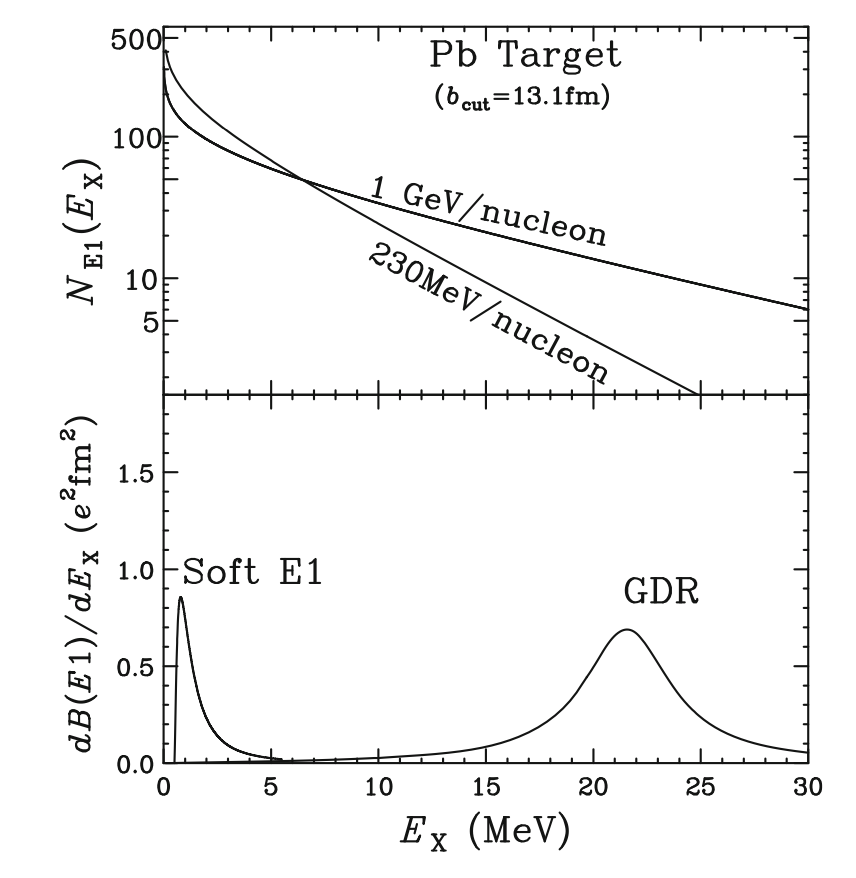
\includegraphics[width=8cm]{chapter2/Virtual_Photon.png}
    \caption[Virtual Photon Spectra and E1 Modes]{Virtual photon spectra and E1 modes. \cite{Nakamura23}}
    \label{fig:Virtual_Photon}
\end{figure}

Another important strangth of Coulomb dissociation is, E1 reduced transition probability is associated with the geometrical information of the two neutron halo nucleus. The non-energy weighted cluster sum rule from Esbensen et at. \cite{Esbensen} can be adopted as,
\begin{align}
    B(E1) &= \int_{-\infty}^{\infty} \frac{dB(E1)}{dE_x}dE_x \notag \\
        &= \frac{3}{\pi} \bigg(\frac{Z e}{A}\bigg)^2 \langle r^2_{c-nn} \rangle \notag \\
        &= \frac{3}{4 \pi} \bigg(\frac{Z e}{A}\bigg)^2 \langle \vec{r_1}^2 + \vec{r_2}^2 + 2 \vec{r_1} \cdot \vec{r_2} \rangle \notag \\
        &= \frac{3}{4 \pi} \bigg(\frac{Z e}{A}\bigg)^2 \langle \vec{r_1}^2 + \vec{r_2}^2 + 2\vec{r_1} \vec{r_2} \cos \theta_{12} \rangle
\end{align}
where $\vec{r_1}$ and $\vec{r_2}$ are neutron position vectors with respect to the core, and $r_{c-nn}$ is the distance between the core and the center of two neutrons. $\theta_{12}$ is the opening angle between two neutrons. From this formula, the dineutron correlation can be extracted by measuring the E1 reduced transition probability. 

\section{Invariant Mass Method}
To reconstruct the excited state of ${}^{17}$B at target, invariant mass method is used. Since ${}^{17}$B has no bound excited state and its two neutron separation energy $S_{2n}$ is very small, the dissociation process occurs very quickly. In this case, the invariant mass method is a useful tool to reconstruct the intermediate excited state of the system by measuring the momentum and energy of all of the fragments. The invariant mass of the excited state $M*$ is defined as
\begin{align}
    M^* &= \sqrt{\bigg(\sum_{i} E_i\bigg)^2 - \bigg(\sum_{i}\vec{P}_i \bigg)^2} 
\end{align}
where $E_i$ and $\vec{P}_i$ are the energy and momentum of the fragment $i$ respectively. In this experiment, the excited state of ${}^{17}$B is reconstructed by measuring the momentum and energy of ${}^{15}$B and two neutrons. The relative energy $E_{rel}$ between ${}^{15}$B and two neutron can be written with the invariant mass as
\begin{align}
    E_{rel} &= M({}^{17}\text{B}^*) - (m_{{}^{15}\text{B}} + m_n + m_n)
\end{align}
where $m_{{}^{15}\text{B}}$, $m_n$ and $m_n$ are the mass of ${}^{15}$B and two neutrons respectively. The relative energy $E_{rel}$ is related to the excitation energy $E_x$ of ${}^{17}$B and neutron separation energy $S_{2n}$ as
\begin{align}
    E_{rel} &= E_x - S_{2n}
\end{align}
Figure 2.3 shows the schematic representation of the invariant mass method. 
\begin{figure}[t]
    \centering
    \setlength{\unitlength}{1mm}
    \begin{picture}(60,40)
        \put(6,15){$E_x$}
        \put(16,1){${}^{17}$B}
        \put(18,31){$M^*$}
        \put(49,11){${}^{15}$B + n + n}
        \put(29,18){$E_{rel}$}
        \put(33,4){$S_{2n}$}
        %\put(10,0){\dashbox{dash-len}}}
        \thicklines
        \put(10,30){\line(1,0){20}}
        \put(10,0){\line(1,0){20}}
        \put(50,10){\line(1,0){20}}
        \put(20,5){\vector(0,1){24}}
        \put(31,29){\vector(1,-1){18}}
        \thinlines
        \multiput(26,10)(1.2,0){20}{\line(1,0){0.8}}
        \multiput(28,0)(1.2,0){10}{\line(1,0){0.8}}
        \put(28,20){\vector(0,1){10}}
        \put(28,20){\vector(0,-1){10}}
        \put(12,20){\vector(0,1){10}}
        \put(12,20){\vector(0,-1){20}}
        \put(32,5){\vector(0,1){5}}
        \put(32,5){\vector(0,-1){5}}
        
    \end{picture}
    \caption{Schematic representation of the invariant mass method} 
\end{figure}

\section{Extracting Coulomb Excitation}
We need to extract only the Coulomb dissociation events from the experimental data. It is unrealistic to directly know which reaction occurs in the target. So we need to use few method to extract only the coulomb dissociation events from all the ${}^{17}\text{B} \to {}^{15}\text{B} + 2n$ event. In this thesis, we used two methods to extract the Coulomb dissociation events. The first method is the $\Gamma$ factor method and the second method is the $\theta_{cut}$ method.

\subsection{$\Gamma$ factor method}
Even though the reaction with lead target is dominant Coulomb interaction, there are still some nuclear interaction. So, we need to extract only the Coulomb dissociation events by subtracting the nuclear interaction events. The reaction with carbon target is usually dominated by nuclear interaction. So, we can extract the Coulomb dissociation cross section by subtracting the cross section of carbon target from the cross section of lead target. Using this method, we can extract the Coulomb dissociation cross section as follows.

\begin{align}
    \sigma_{CD} = \sigma(Pb) - \Gamma \sigma(C),
\end{align}
Where $\Gamma$ is the scaling factor for the nuclear interaction contribution. In this experiment, we used $\Gamma = 2.385$ value from calculation. \cite{Ogata}

\section{Scattering angle}

\begin{figure}
    \centering
    \setlength{\unitlength}{1mm}
    \begin{picture}(100,40)
        
    \end{picture}
\end{figure}

\begin{align}
    \vec{P_{in}} = \vec{P_{{}^{17}B}} \\
    \vec{P_{out}} = \vec{P_{{}^{15}B}} + \vec{P_{n_1}} + \vec{P_{n_2}}\\
    \cos \theta_{lab} = \frac{\vec{P_{in}} \cdot \vec{P_{out}}}{|\vec{P_{in}}||\vec{P_{out}}|}
\end{align}
Lorentz transformation
\begin{align}
    \begin{pmatrix}
        E_{\text{CM}} \\
        \vec{P_{\text{CM}}^{\parallel}} \\
        \vec{P_{\text{CM}}^{\perp}} \\
    \end{pmatrix}
    =
    \begin{pmatrix}
        \gamma & -\gamma \beta_{cm} & 0 \\
        -\gamma \beta_{cm} & \gamma & 0 \\
        0 & 0 & 1 \\
    \end{pmatrix}
    \begin{pmatrix}
        E_{\text{lab}} \\
        \vec{P_{\text{lab}}^{\parallel}} \\
        \vec{P_{\text{lab}}^{\perp}} \\
    \end{pmatrix} 
\end{align}


For fixed target, $\vec{P_{tgt}}$ is zero, so $E_{tgt} = m_{tgt}$
\begin{align}
    \beta_{cm} = \frac{\vec{P_{in}}}{E_{in} + E_{tgt}} = \frac{\vec{P_{in}}}{E_{in} + m_{tgt}}
\end{align}
\begin{align}
    \vec{P_{\parallel}} = \frac{\vec{P_{out}} \cdot \beta_{cm}}{|\beta_{cm}|}\\
    \vec{P_{\perp}} = \vec{P_{out}} - \vec{P_{\parallel}}
\end{align}
After Lorentz transformation, with the Lorentz boosted vector $P^*$, the scattering angle at CM frame can be written as
\begin{align}
    \tan \theta_{cm} = \frac{\vec{P^*_{\perp}}}{P^*_{\parallel}}
\end{align}

\begin{figure}[b]
    \centering
    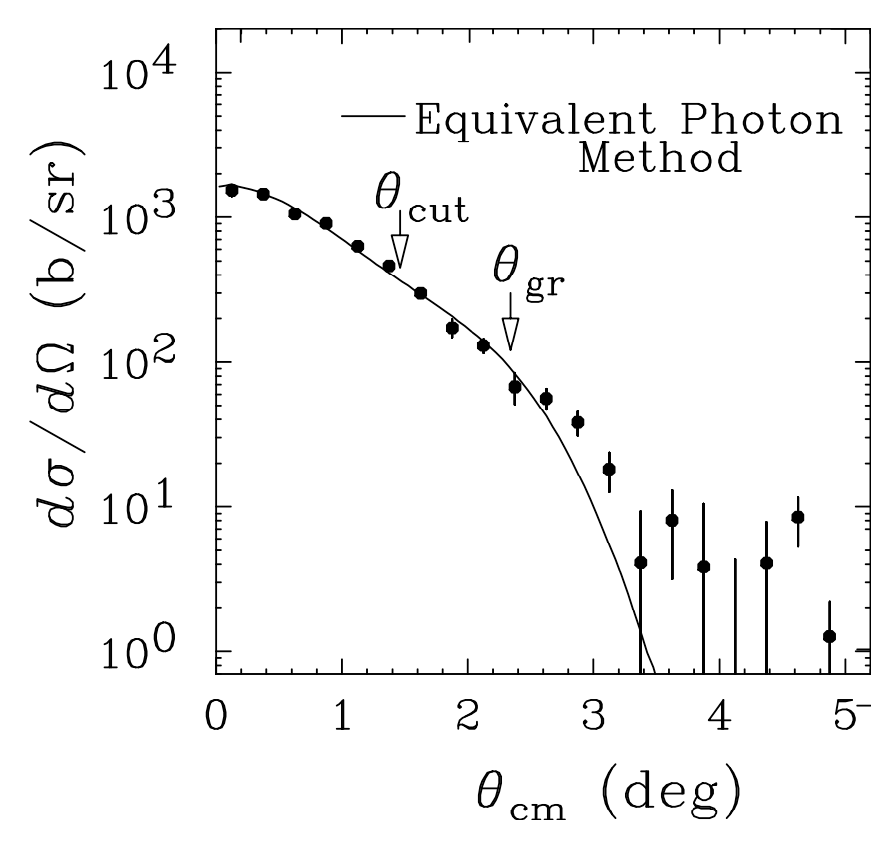
\includegraphics[width=8cm]{chapter2/theta_cut.png}
    \caption[The $\theta_{cut}$ method]{The $\theta_{cut}$ method. \cite{Nakamura11Li}}
\end{figure}
